\tikzset{every picture/.style={line width=0.75pt}} %set default line width to 0.75pt        

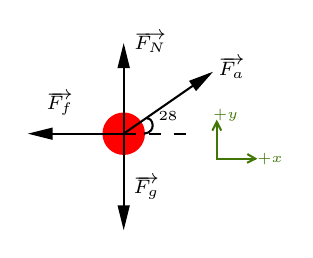
\begin{tikzpicture}[x=0.75pt,y=0.75pt,yscale=-1,xscale=1]
	%uncomment if require: \path (0,300); %set diagram left start at 0, and has height of 300

	%Shape: Ellipse [id:dp7093999861642637] 
	\draw  [color={rgb, 255:red, 255; green, 0; blue, 0 }  ,draw opacity=1 ][fill={rgb, 255:red, 255; green, 0; blue, 0 }  ,fill opacity=1 ] (186.23,101.02) .. controls (186.23,95.64) and (190.58,91.29) .. (195.96,91.29) .. controls (201.33,91.29) and (205.69,95.64) .. (205.69,101.02) .. controls (205.69,106.39) and (201.33,110.75) .. (195.96,110.75) .. controls (190.58,110.75) and (186.23,106.39) .. (186.23,101.02) -- cycle ;
	%Straight Lines [id:da6548156036946866] 
	\draw [line width=0.75]    (195.96,101.02) -- (195.96,59.41) ;
	\draw [shift={(195.96,57.41)}, rotate = 90] [fill={rgb, 255:red, 0; green, 0; blue, 0 }  ][line width=0.08]  [draw opacity=0] (12,-3) -- (0,0) -- (12,3) -- cycle    ;
	%Straight Lines [id:da7473835217170912] 
	\draw [line width=0.75]    (195.96,101.02) -- (237.34,72.33) ;
	\draw [shift={(238.98,71.19)}, rotate = 145.27] [fill={rgb, 255:red, 0; green, 0; blue, 0 }  ][line width=0.08]  [draw opacity=0] (12,-3) -- (0,0) -- (12,3) -- cycle    ;
	%Straight Lines [id:da852905721719166] 
	\draw [line width=0.75]    (195.96,101.02) -- (151.75,101.02) ;
	\draw [shift={(149.75,101.02)}, rotate = 360] [fill={rgb, 255:red, 0; green, 0; blue, 0 }  ][line width=0.08]  [draw opacity=0] (12,-3) -- (0,0) -- (12,3) -- cycle    ;
	%Straight Lines [id:da7879707425395328] 
	\draw [line width=0.75]    (195.96,101.02) -- (195.96,145.5) ;
	\draw [shift={(195.96,147.5)}, rotate = 270] [fill={rgb, 255:red, 0; green, 0; blue, 0 }  ][line width=0.08]  [draw opacity=0] (12,-3) -- (0,0) -- (12,3) -- cycle    ;
	%Shape: Right Angle [id:dp015604455251778004] 
	\draw  [color={rgb, 255:red, 65; green, 117; blue, 5 }  ,draw opacity=1 ] (259.53,113.15) -- (240.84,113.15) -- (240.84,95.32) ;
	\draw  [color={rgb, 255:red, 65; green, 117; blue, 5 }  ,draw opacity=1 ] (242.96,99.54) -- (240.81,95.35) -- (238.68,99.55) ;
	\draw  [color={rgb, 255:red, 65; green, 117; blue, 5 }  ,draw opacity=1 ] (255.4,115.02) -- (259.34,113.06) -- (255.53,110.83) ;

	%Curve Lines [id:da9919868327074761] 
	\draw    (205.69,101.02) .. controls (212.28,100.3) and (209.87,92.89) .. (207.11,93.76) ;
	%Straight Lines [id:da6820111378004245] 
	\draw  [dash pattern={on 4.5pt off 4.5pt}]  (195.96,101.02) -- (225.89,101.02) ;

	% Text Node
	\draw (199.61,50.44) node [anchor=north west][inner sep=0.75pt]  [font=\scriptsize] [align=left] {$\displaystyle \overrightarrow{F_{N}}$};
	% Text Node
	\draw (240.22,62.76) node [anchor=north west][inner sep=0.75pt]  [font=\scriptsize] [align=left] {$\displaystyle \overrightarrow{F_{a}}$};
	% Text Node
	\draw (157.27,79.34) node [anchor=north west][inner sep=0.75pt]  [font=\scriptsize] [align=left] {$\displaystyle \overrightarrow{F_{f}}$};
	% Text Node
	\draw (199.25,119.91) node [anchor=north west][inner sep=0.75pt]  [font=\scriptsize] [align=left] {$\displaystyle \overrightarrow{F_{g}}$};
	% Text Node
	\draw (211.24,88.8) node [anchor=north west][inner sep=0.75pt]  [font=\tiny] [align=left] {$\displaystyle 28\degree $};
	% Text Node
	\draw (258.87,108.89) node [anchor=north west][inner sep=0.75pt]  [font=\tiny,color={rgb, 255:red, 65; green, 117; blue, 5 }  ,opacity=1 ] [align=left] {$\displaystyle +x$};
	% Text Node
	\draw (237.51,87.53) node [anchor=north west][inner sep=0.75pt]  [font=\tiny,color={rgb, 255:red, 65; green, 117; blue, 5 }  ,opacity=1 ] [align=left] {$\displaystyle +y$};


\end{tikzpicture}